% T402 Payment Sequence Diagram - Standalone TikZ
% Compile with: pdflatex payment-sequence.tex

\documentclass[tikz,border=10pt]{standalone}
\usepackage{tikz}
\usetikzlibrary{arrows.meta, positioning, calc}
\usepackage{xcolor}

% Define colors
\definecolor{t402blue}{HTML}{3B82F6}
\definecolor{t402green}{HTML}{10B981}
\definecolor{t402purple}{HTML}{8B5CF6}
\definecolor{t402gray}{HTML}{6B7280}
\definecolor{t402orange}{HTML}{F59E0B}
\definecolor{t402red}{HTML}{EF4444}

\begin{document}
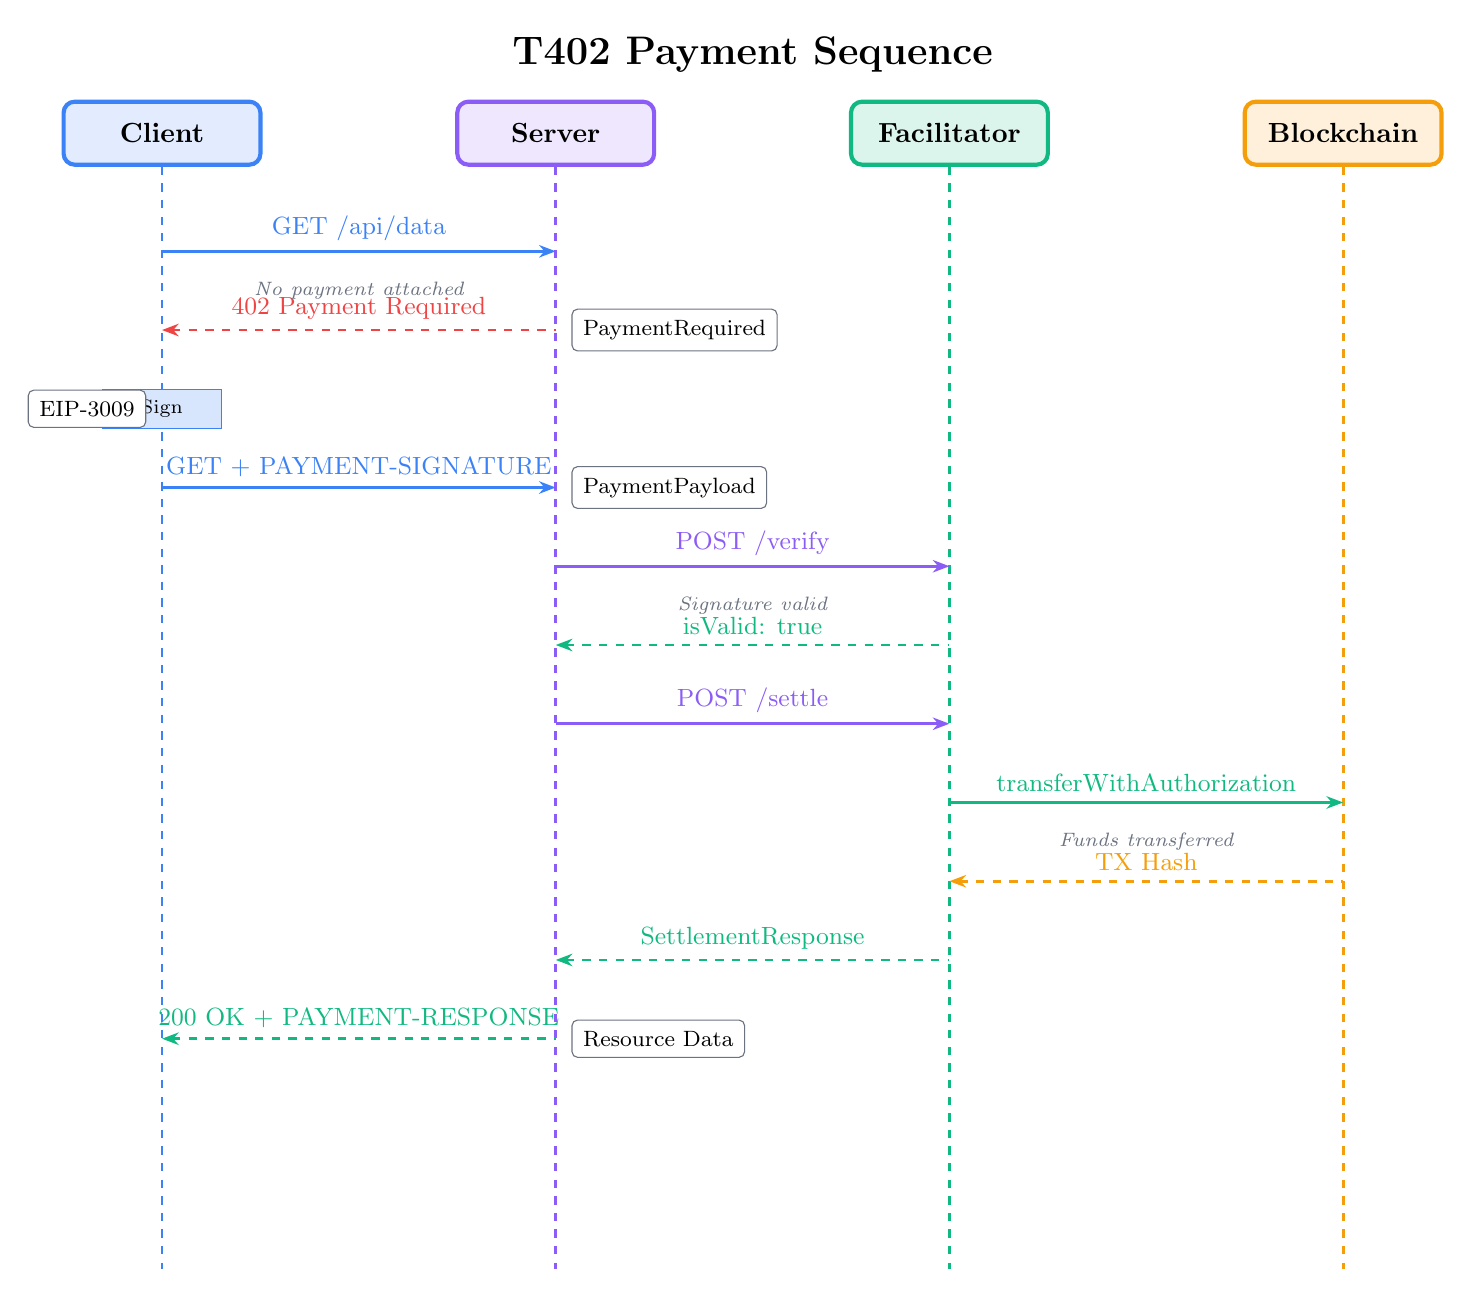
\begin{tikzpicture}[
    actor/.style={
        rectangle,
        rounded corners=4pt,
        minimum width=2.5cm,
        minimum height=0.8cm,
        draw=#1,
        line width=1.5pt,
        fill=#1!15,
        font=\bfseries
    },
    lifeline/.style={
        dashed,
        line width=1pt,
        #1
    },
    message/.style={
        ->,
        >={Stealth[length=6pt]},
        line width=1pt,
        #1
    },
    return/.style={
        <-,
        >={Stealth[length=6pt]},
        line width=1pt,
        dashed,
        #1
    },
    note/.style={
        rectangle,
        rounded corners=2pt,
        draw=t402gray,
        fill=white,
        font=\footnotesize,
        inner sep=4pt
    },
    action/.style={
        rectangle,
        minimum width=1.5cm,
        minimum height=0.5cm,
        draw=#1,
        fill=#1!20,
        font=\scriptsize
    }
]

% Actors
\node[actor=t402blue] (client) at (0,0) {Client};
\node[actor=t402purple] (server) at (5,0) {Server};
\node[actor=t402green] (facilitator) at (10,0) {Facilitator};
\node[actor=t402orange] (blockchain) at (15,0) {Blockchain};

% Lifelines
\draw[lifeline=t402blue] (client.south) -- ++(0,-14);
\draw[lifeline=t402purple] (server.south) -- ++(0,-14);
\draw[lifeline=t402green] (facilitator.south) -- ++(0,-14);
\draw[lifeline=t402orange] (blockchain.south) -- ++(0,-14);

% Step 1: Initial Request
\draw[message=t402blue] (0,-1.5) -- node[above, font=\small] {GET /api/data} (5,-1.5);

% Step 2: 402 Response
\draw[return=t402red] (0,-2.5) -- node[above, font=\small] {402 Payment Required} (5,-2.5);
\node[note, right] at (5.2,-2.5) {PaymentRequired};

% Step 3: Sign Payment (local)
\node[action=t402blue] at (0,-3.5) {Sign};
\node[note, left] at (-0.2,-3.5) {EIP-3009};

% Step 4: Request with Payment
\draw[message=t402blue] (0,-4.5) -- node[above, font=\small] {GET + PAYMENT-SIGNATURE} (5,-4.5);
\node[note, right] at (5.2,-4.5) {PaymentPayload};

% Step 5: Verify
\draw[message=t402purple] (5,-5.5) -- node[above, font=\small] {POST /verify} (10,-5.5);

% Step 6: Verify Response
\draw[return=t402green] (5,-6.5) -- node[above, font=\small] {isValid: true} (10,-6.5);

% Step 7: Settle
\draw[message=t402purple] (5,-7.5) -- node[above, font=\small] {POST /settle} (10,-7.5);

% Step 8: On-chain Transaction
\draw[message=t402green] (10,-8.5) -- node[above, font=\small] {transferWithAuthorization} (15,-8.5);

% Step 9: TX Confirmation
\draw[return=t402orange] (10,-9.5) -- node[above, font=\small] {TX Hash} (15,-9.5);

% Step 10: Settlement Response
\draw[return=t402green] (5,-10.5) -- node[above, font=\small] {SettlementResponse} (10,-10.5);

% Step 11: Success Response
\draw[return=t402green] (0,-11.5) -- node[above, font=\small] {200 OK + PAYMENT-RESPONSE} (5,-11.5);
\node[note, right] at (5.2,-11.5) {Resource Data};

% Annotations
\node[font=\scriptsize\itshape, t402gray] at (2.5,-2) {No payment attached};
\node[font=\scriptsize\itshape, t402gray] at (7.5,-6) {Signature valid};
\node[font=\scriptsize\itshape, t402gray] at (12.5,-9) {Funds transferred};

% Title
\node[font=\bfseries\Large] at (7.5,1) {T402 Payment Sequence};

\end{tikzpicture}
\end{document}
